\chapter{Control PC}

\thispagestyle{plain}
\renewcommand{\tablename}{Tabla}

\section{Introducción}

En este capítulo se describirán los subsistemas y modelos creados que permitirán el control del vehículo robótico desde un ordenador. Este ordenador se comunicará con la placa Arduino haciendo uso del puerto serie de esta. Para realizar esta comunicación se decide utilizar el nuevo \textit{Add-On}, \textit{Simulink-Real Time} introducido en la versión R2023b de MATLAB.

\section{Pruebas iniciales comunicación serie.}

Debido a la novedad de esta librería, se decide probar la comunicación con un programa simple que realice dos sumas y encienda dos LEDs. 

El modelo de la figura \ref{fig:PruebaSerie-Arduino} será el que se esté ejecutando en la placa Arduino. El bloque `\textit{Protocol Encoder}' recibirá cuatro señales, procedentes de dos constantes y su suma, y una última que corresponderá a la suma de los dos números recibidos. Para comprobar la recepción de estos se decide añadir dos bloques que detecten si la suma equivale a 5 ó 10 y encienda un LED conectado a dicho puerto. Una vez codificada la información esta se enviará por el puerto seria al ordenador sólo en el caso de que esta sea diferente. Se decide utilizar el `\textit{Enabled Subsystem}' para esto, con el objetivo de no saturar la comunicación.

\begin{figure}[H]
    \centering
    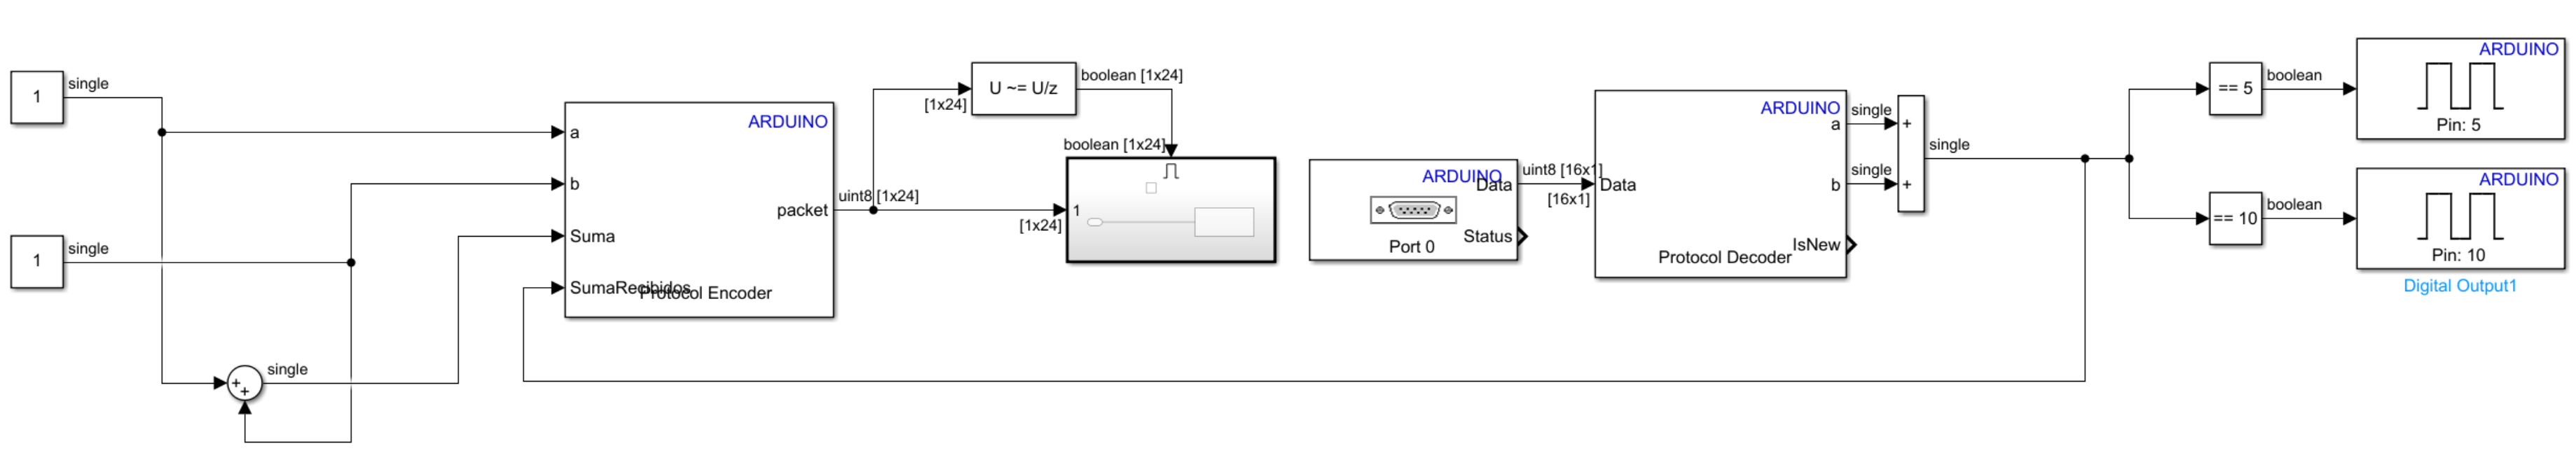
\includegraphics[width=1\linewidth]{imagenes/Simulink - Prueba Serie Arduino PC.png}
    \caption{Modelo prueba serie Arduino.}
    \label{fig:PruebaSerie-Arduino}
\end{figure}

El modelo de la figura \ref{fig:PruebaSerie-PC} será el que se simule en el ordenador. Con él podremos modificar dos constantes que serán enviadas por el puerto serie a la placa Arduino sólo en el caso de que estos valores cambien (al igual que en el modelo anterior). En este modelo no es necesario un bloque `\textit{Protocol Decoder}' ya que el propio `\textit{Serial Receive}' permite configurar el \textit{Header} y \textit{Terminator} y el tipo de datos de la trama. Para dividirlo en cada una de las señales sólo es necesario utilizar un demultiplexor.

\begin{figure}[H]
    \centering
    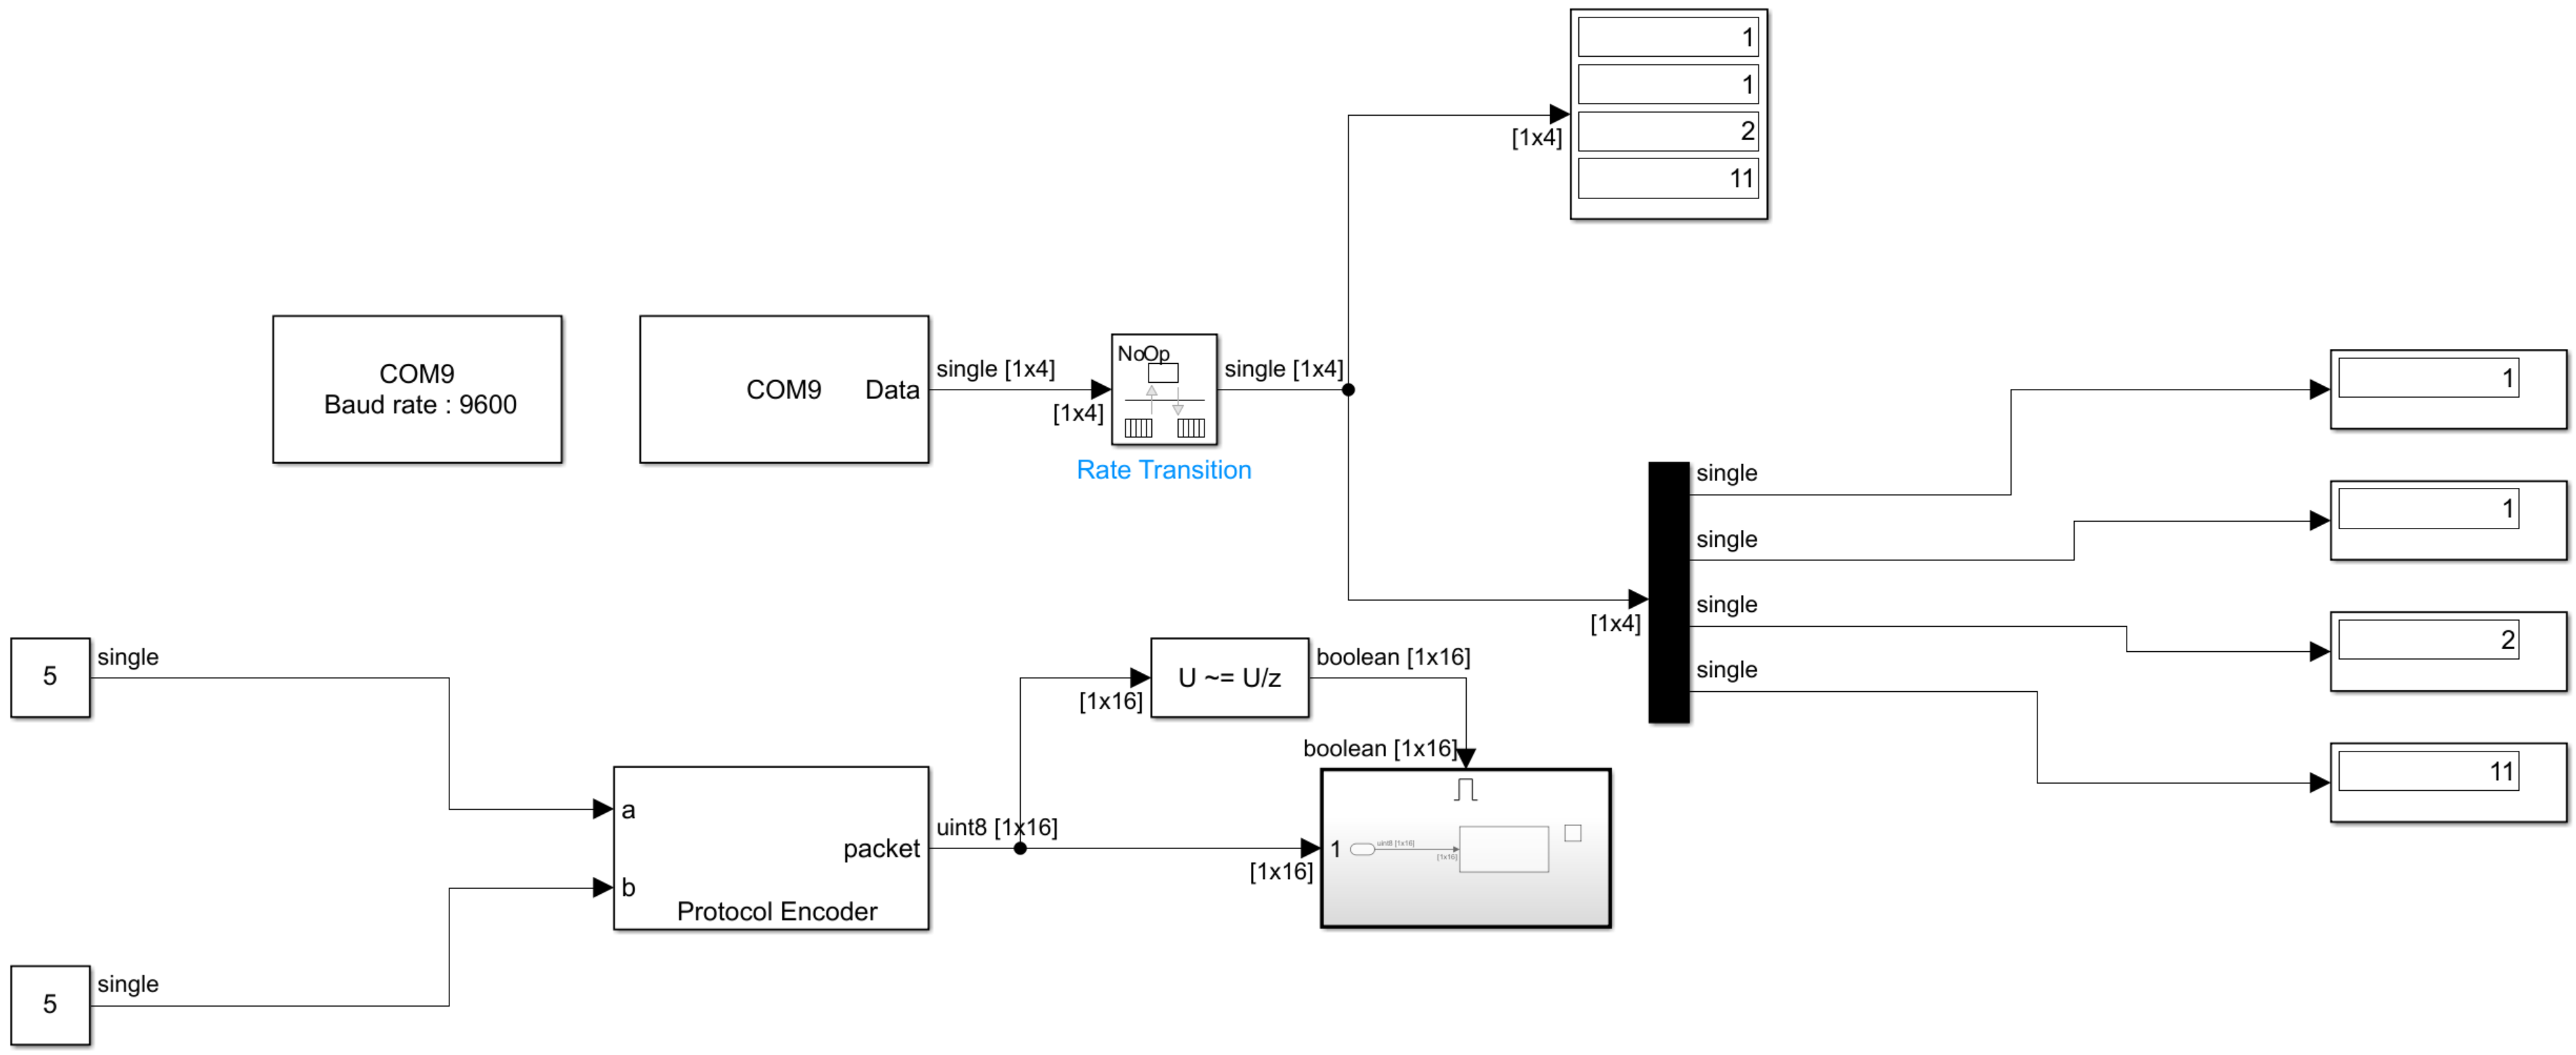
\includegraphics[width=1\linewidth]{imagenes/Simulink - Prueba Serie PC Arduino.png}
    \caption{Modelo prueba serie PC.}
    \label{fig:PruebaSerie-PC}
\end{figure}

Durante la realización de estas pruebas, se identificó la importancia de definir el tamaño del dato recibido por serial. Esta información es del tipo \textit{uint8} y su tamaño lo podremos encontrar en la señal ya empaquetada que se pretende recibir. En este ejemplo el mensaje enviado al PC es de \([1 \times 24]\) y el enviado a la placa Arduino de \([1 \times 16]\).

\section{Subsistemas Simulink}

\subsection{\textit{Send to Arduino}}

Este subsistema recibirá como entradas los parámetros de velocidad lineal y angular así como una señal de \textit{Mode} que determinará si queremos encender u apagar los motores. Esta información será codificada y enviada a la placa Arduino. Para no saturar el canal de comunicación sólo se transmitirá la información en caso de que esta haya cambiado.

\begin{figure}[H]
    \centering
    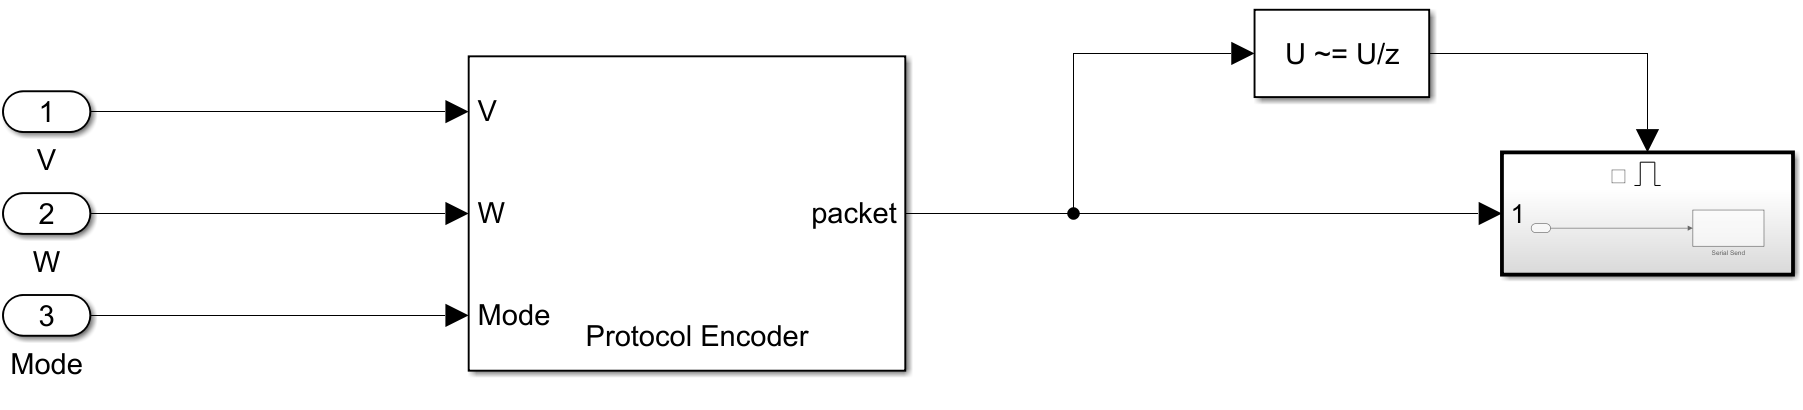
\includegraphics[width=1\linewidth]{imagenes/Simulink - Subsystem - Send to Arduino.png}
    \caption{Subsistema Send to Arduino}
    \label{fig:Subsistema-SendToArduino}
\end{figure}

Con el fin de unificar el método de codificación de las señales durante las comunicaciones en serie se decide que todos los datos sean del tipo \textit{single} y que el orden de los bytes sea \textit{Little endian}. Además todas las tramas de datos se iniciarán con `\textit{START}' y finalizarán con `\textit{END}' Estas configuraciones serán añadidas en el bloque `\textit{Protocol Encoder}' (Figura \ref{fig:Block Parameters-Protocol Encoder PC}), por último el se configurará el bloque `\textit{Serial Send}' para que transmita la información al puerto de comunicación en el que se encuentra conectada la placa Arduino, además no se utilizará ningún \textit{Header} o \textit{Terminator} puesto que estos ya habrán sido añadidos previamente.

\begin{figure}[H]
     \centering
     \begin{subfigure}[c]{0.45\textwidth}
         \centering
         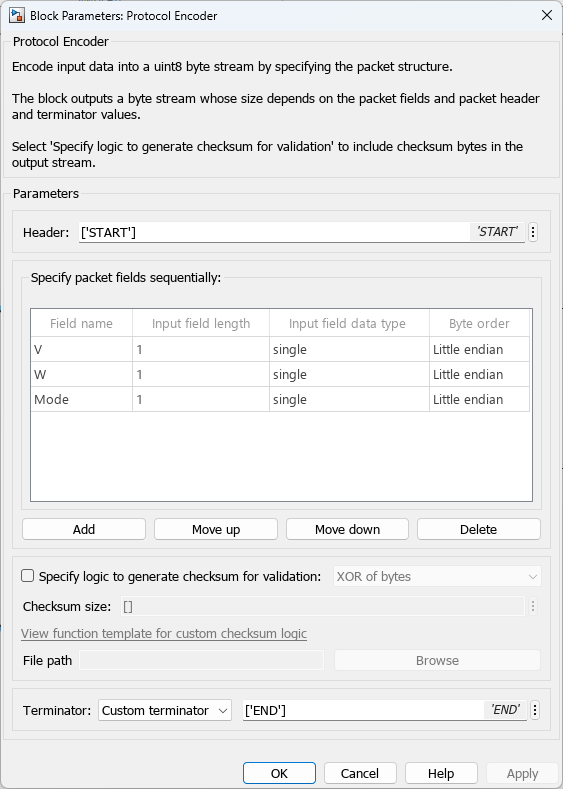
\includegraphics[width=1\textwidth]{imagenes/Simulink - Block Parameters - Protocol Encoder.png}
         \caption{Protocol Encoder}
         \label{fig:Block Parameters-Protocol Encoder PC}
     \end{subfigure}
     \hfill
     \begin{subfigure}[c]{0.45\textwidth}
         \centering
         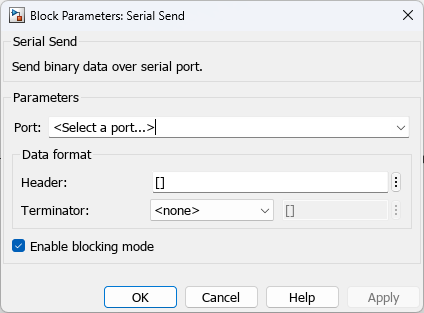
\includegraphics[width=1\textwidth]{imagenes/Simulink - Block Parameters - Serial Send.png}
         \caption{Serial Send}
         \label{fig:Block Parameters-Serial Send}
     \end{subfigure}
        \caption{Parámetros de los bloques}
        \label{fig:enter-label}
\end{figure}

\subsection{\textit{Receive from Arduino}}

Este subsistema se encarga de recibir la información desde la placa, esta incluirá la velocidad lineal y angular y un booleano para motor que indicará la presencia o no de un error en estos. Dicha información se mostrará en los bloques `\textit{Display}' y a su vez será la que se muestre gráficamente en el modelo final (Figura \ref{fig:Simulink - Control PC XBox ROS}).

\begin{figure}[H]
    \centering
    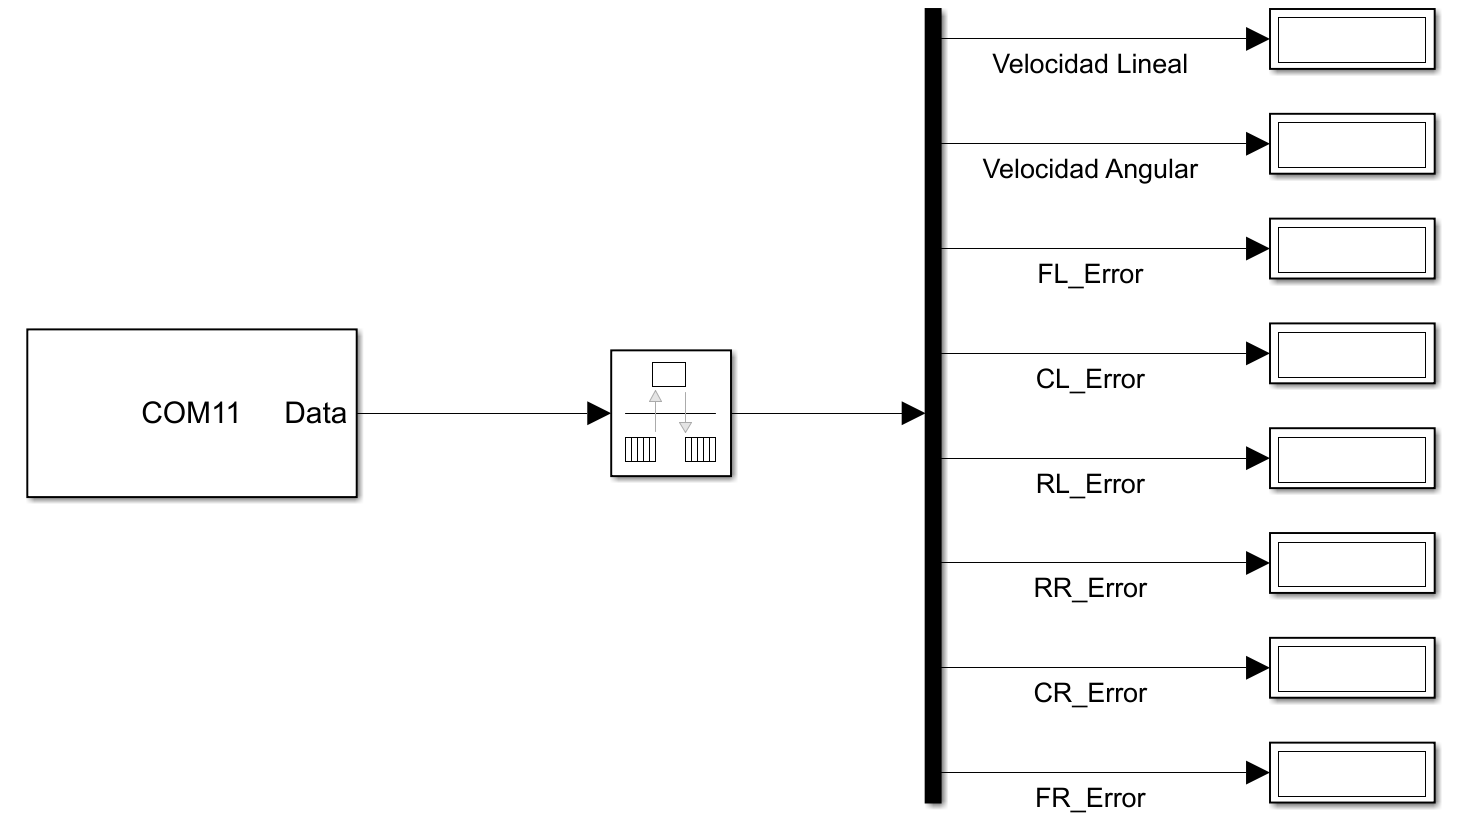
\includegraphics[width=1\linewidth]{imagenes/Simulink - Subsystem - Receive from Arduino.png}
    \caption{Subsistema Receive from Arduino}
    \label{fig:Receive from Arduino}
\end{figure}

Debido a que el bloque `\textit{Serial Receive}' permite configurar el tipo y tamaño del dato recibido, además del \textit{Header} y \textit{Terminator}, no es necesario la utilización de un bloque dedicado íntegramente a la decodificación de la información.

\begin{figure}[H]
    \centering
    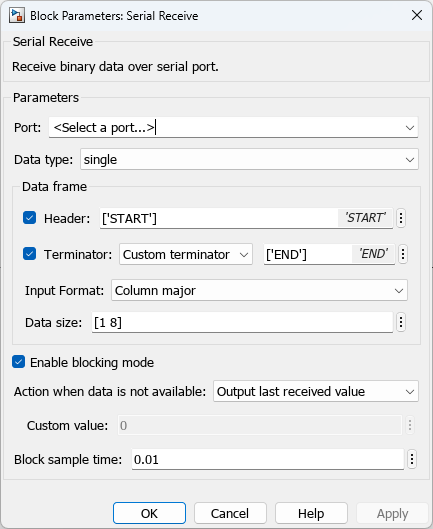
\includegraphics[width=0.5\linewidth]{imagenes/Simulink - Block Parameters - Serial Receive.png}
    \caption{Parámetros del bloque Serial Receive}
    \label{fig:Block Parameters - Serial Receive PC}
\end{figure}

\subsection{\textit{XBox Controller}}

\begin{figure}[H]
    \centering
    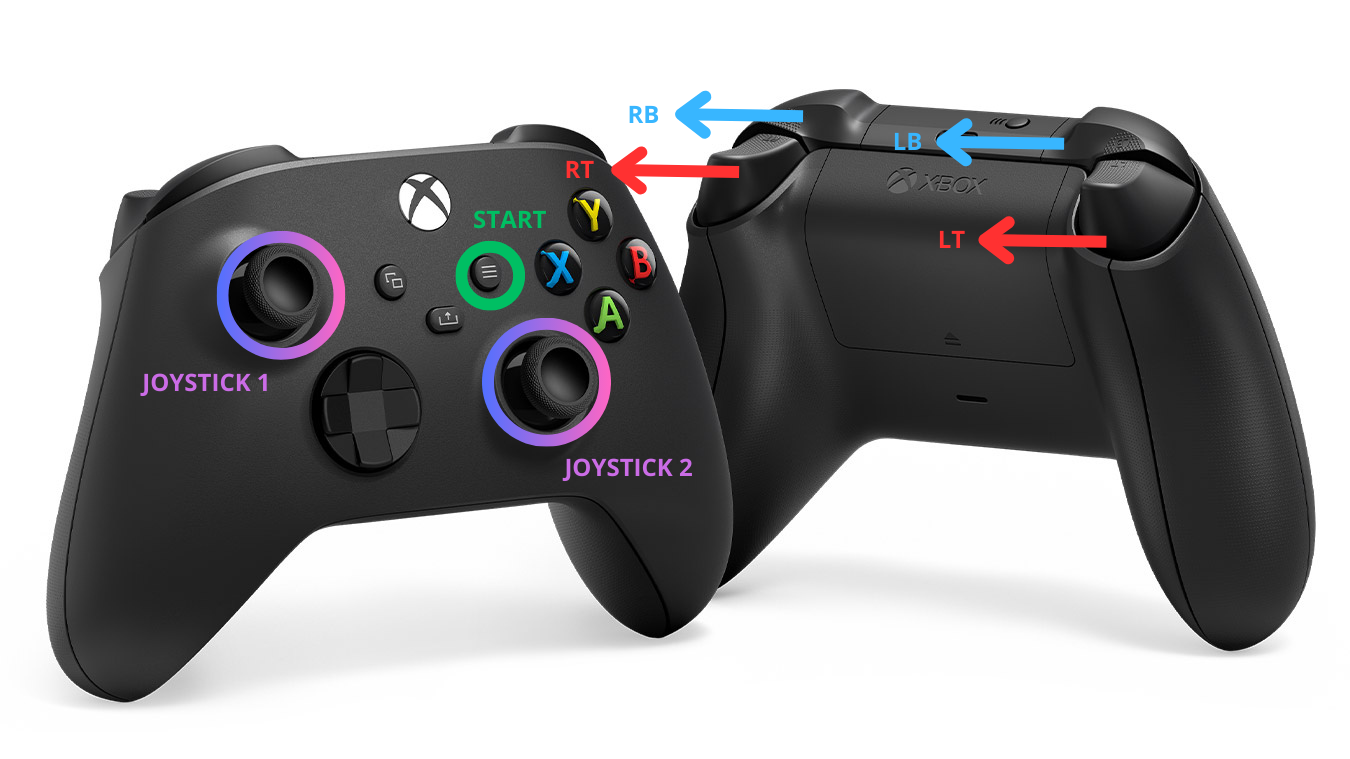
\includegraphics[width=0.75\linewidth]{imagenes/XBox Mando.png}
    \caption{Mando inalámbrico XBox}
    \label{fig:Mando XBox}
\end{figure}

Este subsistema permite controlar de manera inalámbrica el vehículo robótico haciendo uso de un mando de Microsoft (Figura \ref{fig:Mando XBox}). Su bloque principal, \textit{XInput Controller}, se obtiene a partir del \textit{File Exchange} de MathWorks \cite{SimulinkXboxController}. Este bloque informa tanto de las señales los botones y \textit{joysticks}, como del estado de conexión y carga de la batería del mando. 

Sus salidas son:
\begin{itemize}
    \item \textit{Axes}: Vector de seis señales procedentes de los ejes X e Y de cada \textit{joystick} y de los gatillos (RT y LT). Estas señales son del tipo continuas, por lo que previo a su uso, se discretizan haciéndolas pasar por el bloque `\textit{Zero-Hold-Order}'.
    \item \textit{Buttons}: Vector de doce señales de activación (0 ó 1) procedentes de los botones del mando.
    \item \textit{Info}: Vector de tres señales que proporciona información sobre el estado de la conexión bluetooth con el mando y del nivel de batería de este.
\end{itemize}

\begin{figure}[H]
    \centering
    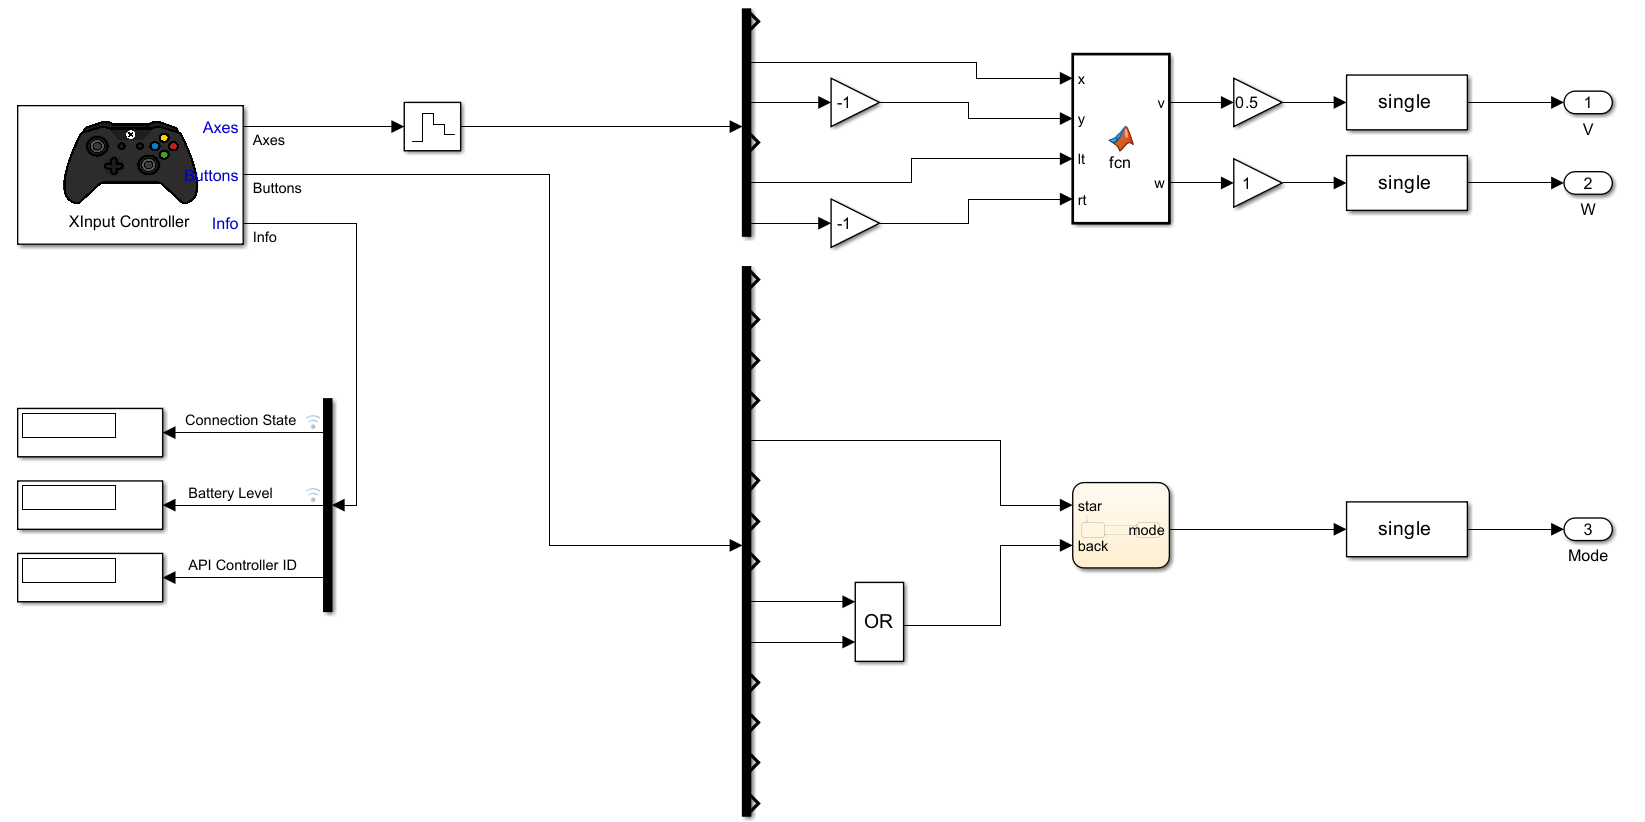
\includegraphics[width=1\linewidth]{imagenes/Simulink - Subsystem - XBox Controller.png}
    \caption{Subsistema XBox Controller}
    \label{fig:Subsistema-XBox Controller}
\end{figure}

Para controlar el encendido y apagado de los motores, se hace uso del bloque `\textit{Chart}'. Este nos permitirá definir los dos estados y las condiciones que se deben de cumplir para que el estado inicial (0) cambie. 

\begin{figure}[H]
    \centering
    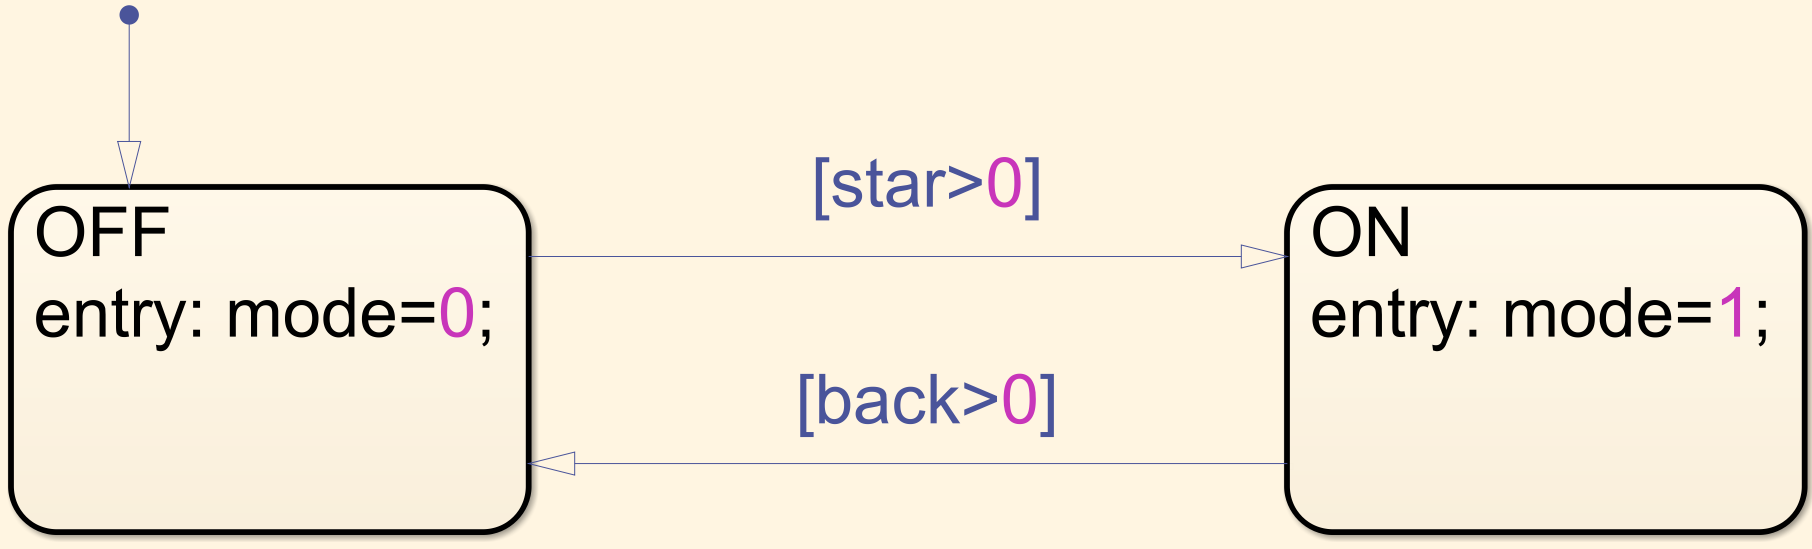
\includegraphics[width=0.5\linewidth]{imagenes/Simulink - Block Parameters - XBox Chart.png}
    \caption{Contenido bloque `\textit{chart}'}
    \label{fig:XBox Controller - Chart}
\end{figure}

Inicialmente el motor se encontrará apagado. Este se encenderá al pulsar el botón `\textit{START}', y se apagará cuando se pulse uno de los botones `RB' ó `LB'.

Por último, para realizar el cálculo de las velocidades linear y angular, se hace uso de la función de MATLAB `XBox - V y W' cuyo código se incluye en el anexo \ref{MATLAB Functions}. Dicha función hará uso de las señales de los ejes X e Y provenientes de ambos \textit{joysticks}.

\subsection{\textit{ROS Publisher}}

Este subsistema se encarga de publicar en la red ROS correspondiente información a tiempo real sobre el estado del vehículo robótico. Este recibirá la velocidad linear y angular, y haciendo uso de esta, mediante el subsistema de odometría explicado más adelante (Figura \ref{fig:Subsistema - Odometria}), se publicará tanto las velocidades como la posición y orientación de este.

\begin{figure}[H]
    \centering
    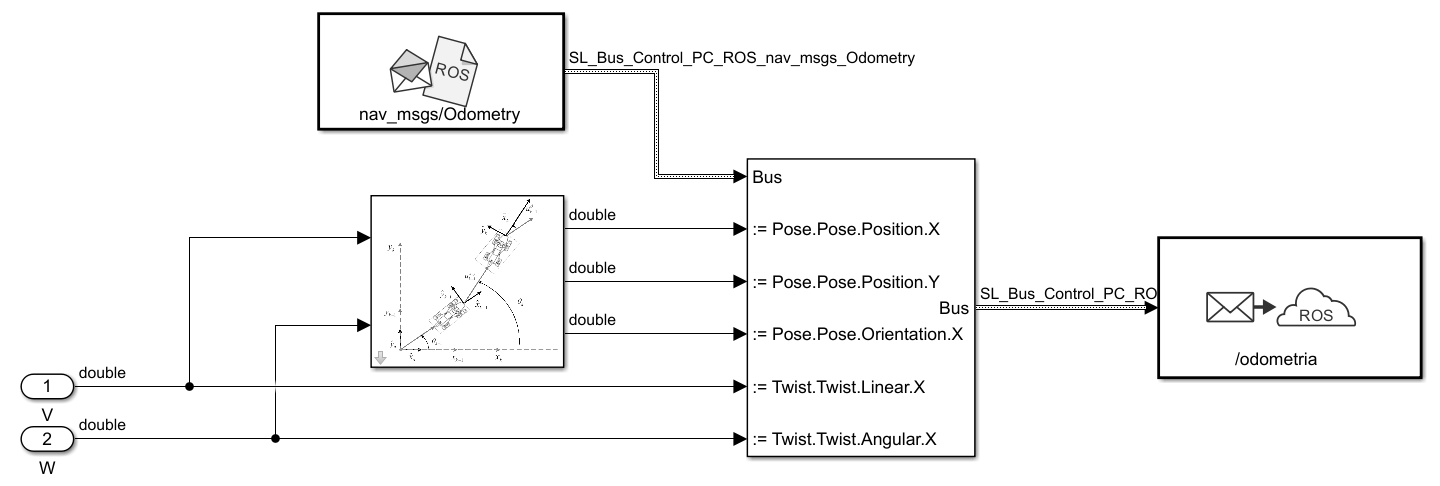
\includegraphics[width=1\linewidth]{imagenes/Simulink - Subsystem - ROS Publisher.png}
    \caption{Subsistema ROS Publisher}
    \label{fig:Subsistema - ROS Publisher}
\end{figure}

\section{Modelo control PC}

Los subsistemas descritos previamente se integran en un modelo que permitirá el control manual del vehículo haciendo uso del mando. A este modelo se le añaden diversos indicadores que permitan conocer el estado del vehículo de manera sencilla. 

\begin{figure}[H]
    \centering
    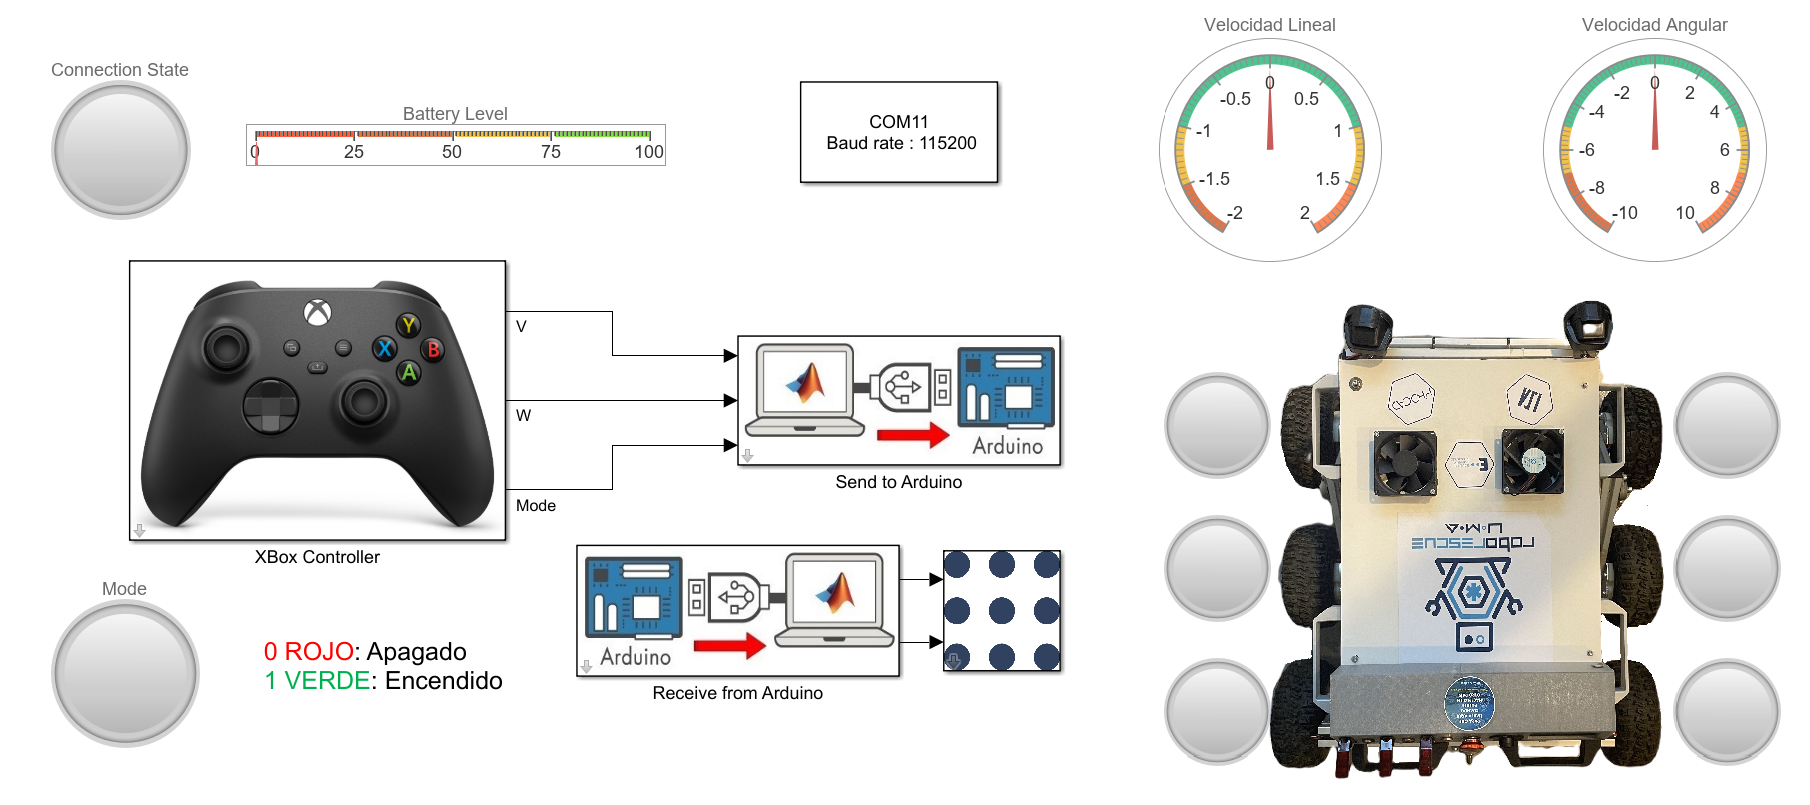
\includegraphics[width=1\linewidth]{imagenes/Simulink - Control PC XBox ROS.png}
    \caption{Modelo Control PC}
    \label{fig:Simulink - Control PC XBox ROS}
\end{figure}

Los indicadores añadidos son:
\begin{itemize}
    \item 6 Lámparas para el vehículo: Estas se encenderán en verde cuando esté funcionando correctamente y cambiarán a rojo cuando se haya detectado algún error en el motor correspondiente.
    \item 1 Indicador Lineal: Conectado a la información del estado de carga de la batería del mando inalámbrico.
    \item 1 Lámpara: Encargada de indicar el estado de la conexión del mando (ROJO: Desconectado, VERDE: Conectado).
    \item 1 Lámpara: Permitirá visualizar si los motores están encendidos (VERDE) o apagados (ROJO).
    \item 2 Indicadores: Conectados a las señales de velocidad linear y angular.
\end{itemize}

%\blankpage